\section{Reproducibility and Detailed Measurements}\label{app:repro}
\paragraph{Cohorts.} The 120 new patients comprise 30 respiratory, 20 cardiovascular, 20 digestive, 20 neurologic, 15 ear/nose/throat, and 15 systemic cases. Their 24 deep trajectories comprise 6, 2, 4, 6, 3, and 3 respectively, with 4--15 updates per case. Each disease has five endpoint patients, but the deep subset is not one case per disease. No exact fact-set overlap with prior cohorts was found, ignoring age and sex. This is an identity check, not a test for simulator-level overlap or pretraining contamination.

\paragraph{Counts.} The completed continuation produced 1,488 natural/input-control observations: 800 main 1.7B observations, 24 No-counterfactual observations, 120 presentation controls, 96 empty-input/candidate-order controls, and 448 4B observations. These include training measurements and repeated conditions; they are not independent patient counts. In addition there are 672 active intervention conditions and 48 zero controls. The present case synthesis adds no model calls. All inference was local, with zero API expenditure.

\paragraph{Architecture and runtime.} Qwen3-1.7B has 28 layers, hidden size 2048, 16 query heads, and eight key/value heads. The 4B configuration has 36 layers, hidden size 2560, 32 query heads, and eight key/value heads; its existing 8-bit quantization uses group size 128. Floating parameters use FP16. Model inference uses MLX on an Apple M2 Pro with 32 GB shared memory; statistical analyses use Python, NumPy, SciPy, and scikit-learn. Recorded manifests retain source and weight hashes. Greedy continuations and teacher-forced candidate scoring use the same evidence and candidate vocabulary. No model parameter is updated.

\paragraph{Readout objective.} Let $Z$ be the matrix of centered, normalized training states at one layer, and $Y$ the one-hot label matrix. We compute
\begin{equation}
 W=Z^\top(ZZ^\top+\lambda I)^{-1}(Y-\bar Y),
\end{equation}
with $b=\bar Y$ and $\lambda=0.1$. Heads are fitted separately for every layer. A separate head for each input presentation avoids silently treating cross-layout readout failure as missing information. Presentation follow-up readouts are evaluated with the original panel head and therefore measure transfer under a changed layout. Endpoint 4B final-layer accuracies at $\lambda=0.01,0.1,1$ are 92.5\%, 91.7\%, and 89.2\%. No test-prefix labels enter fitting.

\paragraph{Internal computation.} For each layer, we save residual input $h^{in}$, attention increment $a$, post-attention state $h^{attn}$, MLP increment $m$, and residual output $h^{out}$. We check $h^{attn}=h^{in}+a$ and $h^{out}=h^{attn}+m$, and continuity into the next layer. Projecting these additive terms through a fixed linear disease contrast decomposes the readout margin algebraically; it does not causally attribute medical reasoning to attention or MLP.

\paragraph{Attention.} The 1.7B endpoint atlas contains 107,520 patient--presentation--layer--head rows ($120\times2\times28\times16$). It measures the diagnostic anchor's attention toward known facts, unknown fields, candidates, and other prompt tokens. Layers 21--28 average known-fact mass is 4.23\% for append and 2.92\% for the original panel; candidate mass is 21.98\% and 15.44\%. The remaining mass includes instructions and formatting and must not be interpreted as medically irrelevant. Per-token-normalized masses are also retained. The full all-position attention tensor is not part of the current capture.

\paragraph{Exact instruction text.} The shared system instruction is:
\begin{quote}\small
You are analyzing a synthetic patient record for research. Compare the listed diagnoses using only the cumulative findings shown. Distinguish past medical history from the current presentation. Missing information is unknown. Some recorded ordinal scales have unspecified endpoint meanings; do not invent a clinical interpretation for their endpoints.
\end{quote}
The panel adds: ``Fixed questionnaire. Unknown means not available; it does not mean No.'' The common response instruction is:
\begin{quote}\small
Select the best-supported candidate for the current presentation at this point. Choose one listed diagnosis even if evidence is incomplete. Complete the JSON object with exactly one candidate diagnosis copied verbatim from the list. Do not abbreviate or add an explanation. The output must have the form \texttt{\{"diagnosis":"exact candidate diagnosis"\}}.
\end{quote}
The chat template uses \texttt{enable\_thinking=False}; the scored assistant prefix is \texttt{\{"diagnosis":"}. Append input includes source evidence-group identifiers; the panel uses the fixed question list. Known-field markers and identifiers are part of the measured presentation, so we do not assume purely semantic equivalence of the complete prompt strings.

\paragraph{Intervention sites and output scores.} Anchor interventions modify only the final prompt position. All-continuation interventions modify the same layer at each scored continuation position, including disease-name and formatting positions, with the local state norm determining displacement magnitude. Thus an all-continuation effect may act directly on disease-name generation, rather than on a single stored pre-answer belief. Character offsets split name and formatting tokens; tokens spanning a boundary count as name tokens. Both full-49 and sampled-24 competitor contrasts are retained. Same-first-token selectivity applies to 13/24 cases and is secondary.

\paragraph{Numerical checks.} All 48 intervention prefixes pass stability checks; none is excluded. Zero interventions preserve outputs exactly. Maximum relative RMS errors in attention reconstruction are $2.523\times10^{-4}$ (1.7B) and $2.480\times10^{-4}$ (4B). Maximum cached-versus-full sequence log-score errors are 0.01727 and 0.03084. These are implementation tolerances, not statistical error bars. Model weights are unchanged by hash before and after inference. All 120 presentation-control prompts were reconstructed with exact input-ID and token-group matches. A metadata discrepancy affecting the recorded baseline descriptor for append-with-24-candidates was documented; actual saved prompts and scores remain intact.

\paragraph{Analysis chronology.} Fixed-panel measurement and disease-direction experiments have frozen protocols and code snapshots. Answer-polarity, second-configuration, presentation, and empty-input controls were added sequentially to investigate observed discrepancies. Continuous update alignment and the exhaustive trajectory taxonomy are post-hoc analyses of existing records. Empty-input score subtraction was specified before those control observations were obtained. The protocols are project-local records, not a public preregistration. No follow-up is described as an independent new patient replication.

\section{Robustness and Scope of the Diagnostic Interface}
\label{app:robust}
\paragraph{Output parsing and string mass.} For 1.7B, the median probability mass of the scored canonical strings is 0.99279 in append and 0.98875 in the panel; 14/120 and 1/120 cases respectively have mass below 0.1. Greedy diagnostic matches are 38/120 and 10/120, versus sequence-ranked 44/120 and 10/120. The native presentation gap therefore also appears in greedy continuations. Sequence-sum and mean-token top choices agree in 90\% and 95\% of cases. For 4B append, greedy matches are 75/120, 117/120 continuations are canonical candidates, median mass is 0.999943, and 119/120 sequence/mean-token top choices agree.

\paragraph{Candidate sets.} The primary 24-class ranking is computed inside a 49-candidate prompt. On the 24 deep cases, changing the prompt itself to 24 candidates gives 6/24 correct panel endpoints and 15/24 append endpoints; reranking the 49-name prompt over those classes gives 4/24 and 12/24. These paired gains have intervals spanning zero and do not remove supervision differences with the probes.

\paragraph{Reference agreement.} Restricting to the 79 cases where the pathology label is also top in the reference differential gives native/readout24 counts of 42/67 for append and 10/77 for the panel, all with denominator 79. This rules out label--differential disagreement as the sole explanation of the observed discrepancy. It does not supply missing intermediate clinical truth.

\paragraph{Disease groups.} Table~\ref{tab:families} shows that the aggregate effect does not require every group to improve internally. Group estimates are descriptive; only five patients represent each disease.
\begin{table}[h]
\centering\small
\begin{tabular}{lrrr}\toprule
Group ($n$) & Native A/P & Probe A/P\\\midrule
Respiratory (30) & 12/9 & 25/28\\
Cardiovascular (20) & 4/1 & 13/19\\
Digestive (20) & 10/0 & 15/20\\
Neurologic (20) & 17/0 & 20/19\\
ENT (15) & 9/0 & 13/15\\
Systemic (15) & 4/4 & 14/11\\\bottomrule
\end{tabular}
\caption{Counts correct in append/panel, same 24 diseases. Probe refers to layer 28.}\label{tab:families}
\end{table}

\paragraph{Input-value controls.} A presence-only representation that hides answer values while retaining known-field positions gives 0/24 native correct diagnoses in the tested panel control. This does not conflict with a supervised field-presence classifier reaching 120/120 on endpoints: the classifier is explicitly trained to exploit the recording pattern, whereas the original model is not. The comparison reinforces the distinction between available predictive information and native use.

\paragraph{Unresolved experiments.} The existing causal test shows a directional effect, not necessity of a natural update. A stronger test would remove the projection of an actual adjacent-prefix state difference onto a direction fixed using different patients and compare same-norm random removal, old-state replacement, and self replacement. A new cohort should confirm layer and dose choices. Other priorities are evidence-pattern-matched cross-diagnosis cases, alternative case sources, precision-matched models, and explicit-thinking conditions. These experiments are not reported as completed.

\section{Ten Contrasting Examples}\label{app:examples}
The following gallery deliberately spans different trajectories; it is illustrative and was selected after analysis. Population counts always include the full 24 preselected patients. The source label supplies a common coordinate for plotting support; it does not prescribe a correct posterior at every partial prefix.

\begin{enumerate}
\item \textbf{Otitis media, 0041136}: the treatment-history group moves append output to the label, which remains selected; the panel keeps COPD despite readable otitis information.
\item \textbf{Pancreatic neoplasm, 0027885}: append output enters the label twice and ultimately selects bronchiolitis, while the endpoint readout selects pancreatic neoplasm.
\item \textbf{Acute dystonic reactions, 0032489}: the append output remains acute laryngitis throughout; the endpoint readout selects the label. This is persistent error without diagnostic oscillation.
\item \textbf{Boerhaave, 0044249}: append output recovers the label at the endpoint, while the final readout selects GERD. This directly challenges the idea of an always-correct hidden answer.
\item \textbf{Pulmonary embolism, 0048692}: append output ends at acute pulmonary edema and the readout at spontaneous pneumothorax. Both channels fail.
\item \textbf{Anemia, 0006854}: append output enters anemia and later returns to pulmonary embolism; the panel ends at anemia. This is a counterexample to uniform panel harm.
\item \textbf{Spontaneous pneumothorax, 0101113}: both append and panel end at the label. Different presentations can converge successfully.
\item \textbf{Guillain--Barr\'{e} syndrome, 0079685}: append output visits several alternatives before eventually reaching the source label. This illustrates delayed acquisition rather than a stable correct diagnosis from the first evidence.
\item \textbf{Pericarditis, 0037913}: append output enters pericarditis, later moves to laryngitis, and ends at Boerhaave, while the final readout selects pericarditis.
\item \textbf{GERD, 0123136}: append output shifts from pulmonary edema to the source label and retains it; panel output ends at COPD. This repeats presentation-dependent separation outside the opening ENT example.
\end{enumerate}
\begin{figure*}[p]
\centering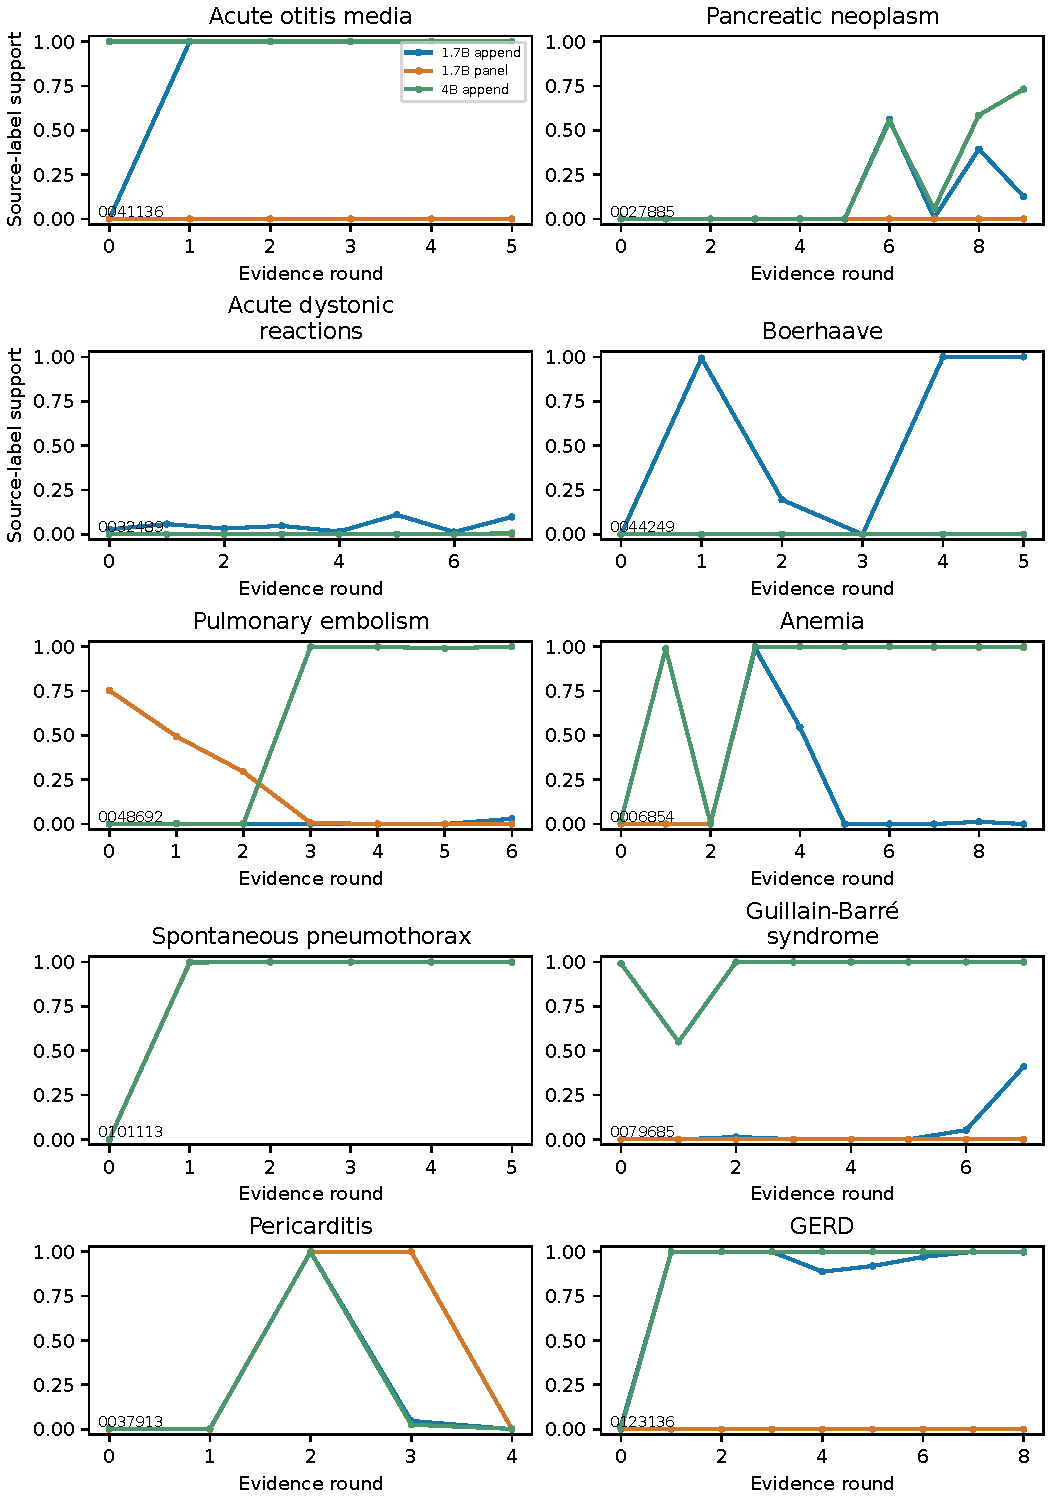
\includegraphics[width=.94\textwidth,height=.84\textheight,keepaspectratio]{figures/case_gallery.pdf}
\caption{Ten contrasting patients. Each line is the model-native relative support for the patient's source-label disease, not a probe probability. Blue: 1.7B append; orange: 1.7B panel; green: 4B append. Source evidence and competing disease identities for every round are given in the complete case appendix.}
\end{figure*}
